% FEEDBACK
%
% !TEX root = ../thesis-main.tex
%
\chapter{Feedback on lexical stress errors}
\label{chap:feedback}

%\cleanchapterquote{You can’t do better design with a computer, but you can speed up your work enormously.}{Wim Crouwel}{(Graphic designer and typographer)}

Since the focus of this thesis is on pronunciation training, not pronunciation assessment (see \cref{sec:capt:systems}), feedback on the errors diagnosed via the methods described in \cref{chap:diagnosis} will be an important component of the proposed CAPT tool. As mentioned in \cref{sec:capt:l2ed}, the particular importance of corrective feedback in pronunciation training is generally acknowledged,
%\citep{Neri2002,Dlaska2013}, 
though much remains to be learned about when and how feedback can be most effective. Therefore, one aim of this thesis is the creation of a feedback generation module for the lexical stress CAPT tool which will offer a variety of possible feedback types, and a Graphical User Interface (GUI) allowing a researcher or instructor to easily switch between feedback types. While it is outside the scope of the thesis to carry out in vivo studies with learners to determine which feedback types are most effective in which situations, the tool will hopefully facilitate such studies going forward. 

%TODO replace?
%In the remainder of this section, various options for the types of feedback that can be generated given a diagnosis of the learner's lexical stress realization are presented, guided by the notion that to maximize its utility in future feedback research, the CAPT tool should offer as wide a variety of feedback options as possible. 

%\textcite{Hattie2007} suggest that feedback in education should help the learner recognize their current learning goals (``Where am I going?''), assess their progress towards them (``How am I going?''), and identify next steps for achieving and moving beyond these goals (``Where to next?'').


%Feedback is important \citep{Neri2002}

%Since our focus is on pronunciation training and not just pronunciation assessment.

%Explicit FB is necessary; learners have trouble identifying their errors when simply asked to listen to what they said \citep{Dlaska2013}

	\begin{figure}[htb]
		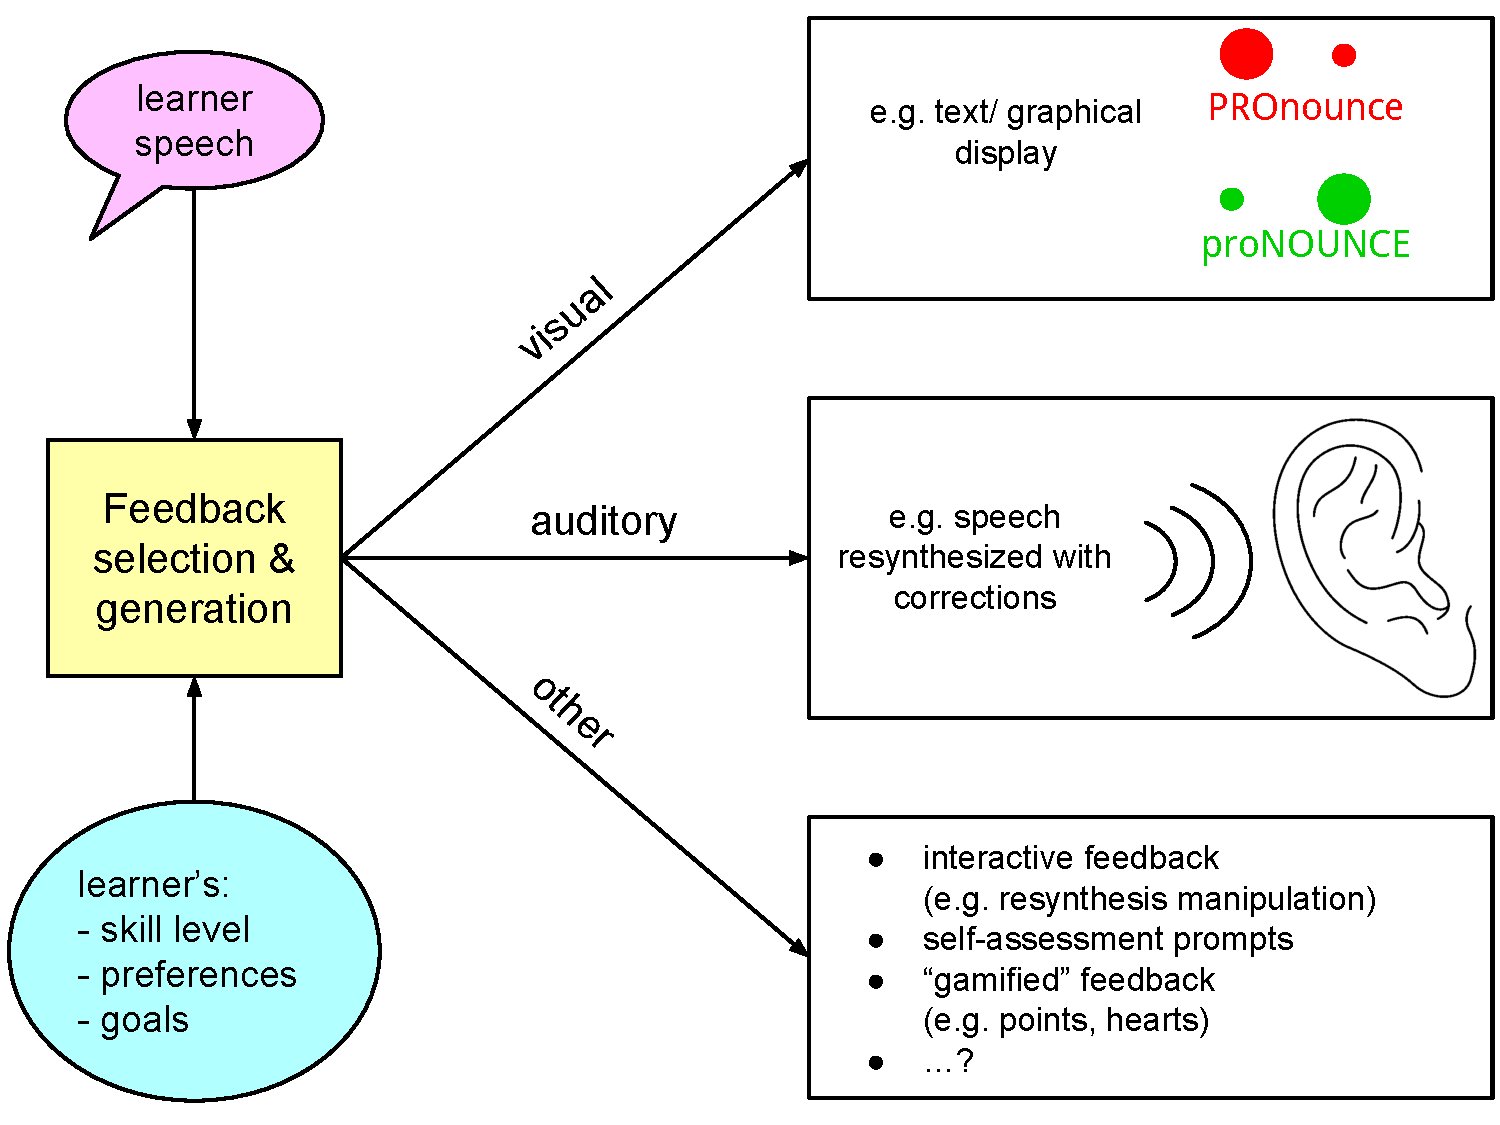
\includegraphics[width=\textwidth]{img/feedback}
		\caption{Delivery of prosody feedback in different modalities.}
		\label{fig:feedback}
	\end{figure}

%\section{Related work}
%\label{sec:fb:related}
%
%	\cite{Sitaram2011}
%	\cite{Bonneau2011}
%	 	\citep{Hattie2007}


\section{Visual feedback}
\label{sec:fb:visual}


	\subsection{Visualizations of the speech signal}
	\label{sec:visual:visualizations}
	In several existing CAPT tools, %such as Snoori \citep{Bonneau2011,Parole2013} and WinPitch LTL \citep{Martin2004}, 
the learner is presented with relatively direct visualizations of the speech signal, such as its waveform (oscillogram) and spectrogram, often with overlays highlighting perceptually relevant properties such as the pitch contour and durations of various parts of the utterance.
	However, as \textcite{Neri2002} point out, waveforms and spectrograms are signal representations designed for speech researchers, not language learners, and the latter may have difficulty understanding these visualizations without the proper training. To research whether this conjecture holds, these direct visualizations must be compared with alternatives in user studies with learners; several options for such alternative visualizations are explored in this section.
	
	
	\subsection{Graphical representations of prosody}
	\label{sec:visual:graphical}
	

	One type of alternative would be a more abstract graphical representation of the lexical stress pattern in the native reference speaker and/or the learner's speech. Classroom materials for pronunciation instruction sometimes represent lexical stress patterns using dots or other shapes, one for each syllable, whose relative sizes indicate each syllable's prominence in the word \citep{Hirschfeld1998}. This type of visualization would be relatively simple to implement, given that the reference or learner utterance can be classified into one of a set of stress patterns \citep{Kim2011,Shahin2012a}. It would also be possible to map the acoustic features of each syllable in the utterance(s) to graphical features of the representative shape, e.g. using size to represent duration, vertical position to represent F0, and darkness to represent intensity. To facilitate studies on which mappings, if any, make this feedback useful to the learner, the researcher-facing GUI should offer control over the different possible mappings.
	
	
	\subsection{Stylized text}
	\label{sec:visual:text}
	
	This is essentially the approach used by \textcite{Sitaram2011}, though they modify the text of each word instead of a more abstract visual representation. As text stylization is also often used in pronunciation instruction materials \citep{Behme-Gissel2005,Hirschfeld2007a}, it would be logical for the CAPT tool to offer text stylization as a feedback option. As with the shapes mentioned above, and following \textcite{Sitaram2011}, it would be interesting to explore the possible mappings between acoustic features and properties of the text of each syllable (e.g. size, weight, underlining/decoration, etc.), with these mappings controllable by the researcher via the GUI.

%Underlining \citep{Hirschfeld2007a}

%Bold + relative position of syllables \citep{Behme-Gissel2005}

\subsection{Other}
\label{sec:visual:other}


	Given some visual representation of the learner's utterance, be it textual or more abstract, visual feedback should also be given on what the learner can do to improve their lexical stress realization. \textcite{Bonneau2011} deliver such feedback in the F0 dimension by displaying arrows which indicate whether the user should raise or lower the pitch of a given syllable to make their realization more like that of the reference speaker, and this is one option for the CAPT tool. Another might be the use of animation to transform the visualization of the learner's (incorrectly realized) utterance into a corresponding visualization of the correct realization, e.g. by growing or shrinking the size of the dot or text for each syllable to visualize the desired change in duration, or showing it moving up or down to convey the desired change in pitch.
	
	
%	Visualizations of the required articulators, such as those displayed in the Fluency pronunciation trainer \citep{Eskenazi2000}, may be helpful for correcting certain segmental errors, but are not likely of much use for correcting lexical stress, and will therefore not be implemented in the proposed tool.

	Implementation of at least one visual feedback type will be of high priority in this work. Stylized text and graphical representations will be explored first. If time allows, animation will be added to convey corrective feedback to the learner.
	
	
\section{Auditory feedback}
\label{sec:fb:auditory}

%Some have speculated that auditory feedback may be more helpful than visual feedback in making learners more aware of lexical stress patterns \citep[p.~3]{Bissiri2009}, so it will be important to address both in the proposed CAPT tool.

In foreign language classrooms, feedback on correct pronunciation is often given implicitly by
%One strategy often used in classrooms is 
%%implicit feedback, i.e. 
allowing the learner to listen to a native speaker's production of the target utterance and/or a recording of their own production.
% while there is no reason not to include the option for this type of implicit feedback in the CAPT tool, it will also be necessary to deliver explicit auditory feedback, as the latter may improve pronunciation more \citep{Dlaska2013} 
	However, 
%as described in \cref{sec:capt:systems} above, 
previous work on delivering lexical stress feedback 
(see \cref{sec:capt:systems}) 
has revealed that learners seem to benefit more from prosodically modified implicit feedback, either in the form of a learner utterance  modified to reflect the ``correct'' prosody of a native reference utterance \citep{Bonneau2011}, or a native utterance modified to place exaggerated emphasis on the stressed syllable \citep{Bissiri2006,Bissiri2009}.
%	%In previous work on delivering %explicit 
%%feedback on lexical stress, as described in \cref{sec:capt:systems}, resynthesis of the learner's utterance has often been performed, where prosodic modifications are applied to make the utterance match the ``correct'' prosody of a reference utterance \citep{Bonneau2011,Bissiri2006,Bissiri2009}. 
%%	Another possibility to be explored follows \citeauthor{Bissiri2009} (\citeyear{Bissiri2006,Bissiri2009}), who found that presenting learners with native model utterances which had been modified to place exaggerated emphasis on the stressed syllable gave positive results. 
%	Therefore, these two types of modification may be implemented in the proposed CAPT tool's feedback module; the prosodic modification capabilities of the Jsnoori program \citep{Parole2013} will be used to transform the given utterance. 
%	If a more generalized model of the native prosody of a given word is developed (see \cref{sec:diag:compare}), it might also be possible to modify a reference (or learner) utterance to match this speaker-independent prosody.
	
	At least one type of audio feedback type will be implemented in the CAPT tool, with the highest-priority option being prosodic modification of the learner's utterance to match a single, manually-selected reference utterance, following \textcite{Bonneau2011}; Jsnoori \citep{Parole2013} will be used to perform this modification. If a generalized lexical stress model is successfully integrated into the diagnostic module (see \cref{sec:diag:compare}), the next highest-priority task will be performing prosodic modification of the learner's utterance based on this model. Emphasizing stressed syllables in the native reference utterance(s) will be of lowest priority. 
 


%\citep{Jilka1998}?

%TODO replace
%	\subsection{Enhanced reference utterance}
%	\label{sec:auditory:enhanced}
%	
%TODO replace
%	\subsection{Resynthesized learner speech}
%	\label{sec:auditory:resynth}
	
	
	
\section{Alternative feedback types}
\label{sec:fb:alternative}

Other options, which will only be explored if time allows, include (in order of priority) feedback encouraging self-assessment and self-correction, metalinguistic feedback, and interactivity. %TODO explain self-regulated learning
 	Self-assessment and self-correction can be encouraged by presenting learners with targeted questionnaires before delivering diagnosis and feedback, e.g. asking learners to listen to their utterance and assess whether they have placed stress on the correct syllable, or 
 	%asking them to listen to an incorrect production (theirs or another speaker's) and 
 	asking how the speaker of an incorrect production could have realized stress properly (``By making the first syllable longer'', etc.). 
	Metalinguistic feedback, e.g. reminding learners %who have made an error 
of the stress rule(s) affecting the target utterance, could be delivered either visually (e.g. text displayed on the screen), auditorily (e.g. playback of an instructor's voice), or both. 
 	Interactivity could be achieved by allowing learners to interact with the resynthesis component to modify the prosody of their utterance, as is done in WinPitch LTL \citep{Martin2004}. %TODO {Snoori too?} 
 	By allowing researchers to easily control which of these feedback options to present to the learner, the tool could facilitate research into the effects of alternative feedback types such as these, which have not yet been adequately studied in CAPT.
 

%TODO replace
%	\subsection{Metalinguistic feedback}
%	\label{sec:alternative:metaling}
%	
%TODO replace
%	\subsection{Interactive feedback}
%	\label{sec:alternative:interactive}
%	
%TODO replace
%	\subsection{Implicit feedback}
%	\label{sec:alternative:implicit}


\section{Summary}
\label{sec:fb:summary}